\documentclass[a4paper]{article}
\usepackage{graphicx}
\topmargin=0.0in
\headheight=0pt
%NAME ADDRESS AND PHOTOGRAPH SECTION

\begin{document}
	\begin{flushleft}
		\textbf{Rohit D Khuspe} \hfill{Phone : +91 7506120970}\\
		3$^{rd}$ year BE, Electronics Engineering\hfill{Email : \underline{rohitkhuspe@gmail.com}}\\
		Fr. Conceicao Rodrigues College of Engieering\\
		Bandra West, Bandstand.\\ 
		
			
	\end{flushleft}

%PHOTO
		\begin{figure}[h]
			\begin{flushright}
				\vspace{-0.5in}
				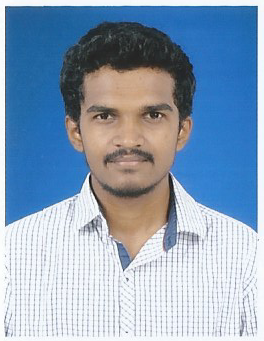
\includegraphics[width=100px]{khuspe.png}
			\end{flushright}
		\end{figure}
	
%OBJECTIVE
		
	\begin{flushleft}
		 	\begin{Large}\textbf{Objective:}\end{Large}  To work in a challenging environment using all my skills\\\hspace{1in} and efforts to explore in Embedded field.\\
 	
%EDUCATION
		 	\begin{Large}\vspace{0.3in}\textbf{Education:}\end{Large}
			 	\vspace{-3mm}
			 	\begin{center}
				 	\begin{tabular}{|l|l|c|c|r|}
					 	\hline
					 	Degree & College/School & University & Passing Year & Percentage\\ \hline
 
						B.E. & Fr.CRCE & MU & 2017 & 7.32(CGPA)\\ \hline
 
					 	12$^{th}$ & I.D.U.B.S. Jr. College & MSBHSC & 2013 & 82.33\\ \hline
 
						10$^{th}$ & Jijamata Vidyamandir & Maharashtra & 2010 & 94\\ \hline

				 	\end{tabular}
			    \end{center}
    
  %PROJECTS
    
  	\begin{Large}\vspace{0.1in}\textbf{Projects:}\end{Large}
  	\begin{enumerate}
  		\item Digital IC Tester using 8051 Microcoltroller
  		\item Autonomous Shopping Robot for e-YIC competition 2016
  		\item Re-energizing the world- ABU Robocon 2016
  	\end{enumerate}
  	
  	
  	
  %TRAINING AND INTRNSHIPS
  
	  	\begin{Large}\vspace{0.1in}\textbf{Training \& Internships:}\end{Large}\\
	  	\begin{itemize}
	  		
	  		\item Intern at E-yantra Summer Internship programme-2016 IIT Bombay
			\item Attended "IoT" workshop organised by ITSA-CRCE in Feb-16
			\item Attended "Level 1 Robotics" workshop organised by CSI-TSEC July-14
		\end{itemize}
		
%ACHIEVEMENTS
			\begin{Large}\vspace{0.1in}\textbf{Achievements:}\end{Large}\\
				\begin{enumerate}
					\item Won e-YIC Competition 2016 and got awarded under "Most Innovative Solution" for "Autonomous Shopping Robot" project.
					\item Secured 21$^{st}$ position in ABU Robocon-2016 competition
				\end{enumerate}
			
%TECHNICAL SKILLS
			\begin{Large}\vspace{0.2in}\textbf{Technical Skills:}\end{Large}\\
			\begin{itemize}
				\item \large\textbf{Programming Languages}
					\begin{enumerate}
						\item C
						\item Embedded C
						\item Assembly Language
					\end{enumerate}
					\item \large\textbf{Microcontrollers}
						\begin{enumerate}
							\item Arduino \{MEGA,UNO,NANO,PRO MINI\} and IDE
							\item Microcontroller 8051 and IDE
							\item Microcontroller Atmega2560 and IDE
							\item Processors 8085 and 8086
						\end{enumerate}
			\end{itemize}
			
%SOFT SKILLS	
			\begin{Large}\vspace{0.1in}\textbf{Soft Skills:}\end{Large}\\
			\begin{enumerate}
				\item Team Working
				\item Creativity
				\item Time Management
				\item Adaptability
			\end{enumerate}
			
%EXTRA-CURRICULAR
				\begin{Large}\vspace{0.1in}\textbf{Extra Curricural Activities:}\end{Large}\\
				\begin{itemize}
					\item Cricket
					\item Swimmimg
				\end{itemize}
				
%CO-CURRICULAR
			\begin{Large}\vspace{0.1in}\textbf{Co-Curricural Activities:}\end{Large}\\
			\begin{enumerate}
					\item Working in Project Cell-CRCE as a Team Member
					\item Was in core team of CRCE-Robocon2016
					\item Volunteered in Team Pravega-CRCE for Student Formula Japan Project 2014
			\end{enumerate}
			
%PERSONAL DETAILS

			\begin{tabular}{ cc }
				\begin{Large}\vspace{0.1in}\textbf{Personal Details:}\end{Large}
				\hfill Fathers Name : & Dhanaji Kaka Khuspe \\ 
				\hfill Mothers Name : & Sunanda Dhanaji Khuspe \\  
				\hfill Sex : & Male   \\ 
				\hfill Date Of Birth : & 23/06/1996  \\
				\hfill Nationality : & Indian  \\
				\hfill Marital Status : & Single
			\end{tabular}
			
%REFERENCE
			\begin{Large}\vspace{0.1in}\textbf{Reference:}\end{Large}
			
%DECLARATION
			
			\begin{Large}\vspace{0.2in}\textbf{Declaration:}\end{Large}
			  \textbf{I hereby declare that the above written}\\\hspace{1.25in}\textbf{particulars are true to the best of my knowledge}\\\hspace{1.25in}\textbf{and belief.}\\
			  
%DATE

				\begin{Large}\vspace{0.1in}\textbf{Date:}\end{Large}
				\hspace{0.68in}24$^{th}$ May, 2016
				
	\end{flushleft}

\end{document}
